\chapter{Exponential sum growth exponents}

\section{Phase functions}

\begin{definition}[Phase function]\label{phase-def}
A \emph{phase function} is a (variable) smooth function $F \colon [1,2] \to \R$.  A phase function $F$ will be called a \emph{model phase function} if there exists a fixed exponent $\sigma > 0$ with the property that
\begin{equation}\label{fpu}
F^{(p+1)}(u) - \frac{d^p}{du^p} u^{-\sigma} = o(1)
\end{equation}
for all (variable) $u \in [1,2]$ and all fixed $p \geq 0$, where $F^{(p+1)}$ denotes the $(p+1)^{\mathrm{st}}$ derivative of $F$.
\end{definition}

For instance, $u \mapsto \log u$ is a model phase function (with $\sigma=1$), and for any fixed $\sigma \neq 1$, $u \mapsto u^{1-\sigma}/(1-\sigma)$ is also a model phase function.  Informally, a model phase function is a function which asymptotically behaves like $u \mapsto \log u$ (for $\sigma = 1$) or $u \mapsto u^{1-\sigma}/(1-\sigma)$ (for $\sigma \neq 1$), up to constants.  This turns out to be a good class for exponential sum estimates, as it is stable under Weyl differencing and Legendre transforms, which show up in the van der Corput A-process and B-process respectively.

Note from Proposition \ref{auto} that the $o(1)$ decay rate in \eqref{fpu} can be made uniform, after passing to a subsequence if necessary.

\section{Exponential sum exponent}

The main purpose of this chapter is to introduce and establish the basic properties of the following exponent function.

\begin{definition}[Exponent sum growth exponent]\label{beta-def}\uses{phase-def}  For any fixed $\alpha \geq 0$, let $\beta(\alpha) \in \R$ denote the least possible (fixed) exponent for which the following claim holds: whenever $N, T \geq 1$ are (variable) quantities with $T$ unbounded and $N = T^{\alpha+o(1)}$, $F$ is a model phase function, and $I \subset [N, 2N]$ is an interval, then
$$ \sum_{n \in I} e(T F(n/N)) \ll T^{\beta(\alpha)+o(1)}.$$
\end{definition}

\python{bound_beta}
\code{Bound_beta}

It is easy to see that the set of possible candidates for $\beta(\alpha)$ is closed (thanks to underspill), non-empty, and bounded from below, so $\beta$ is well-defined as a (fixed) function from $[0,+\infty)$ to $\R$.  Specializing to the logarithmic phase $F(u) = \log u$, and performing a complex conjugation, we see in particular that
\begin{equation}\label{beta-alpha}
    \sum_{n \in I} n^{-iT} \ll T^{\beta(\alpha)+o(1)}
\end{equation}
whenever $T$ is unbounded, $N = T^{\alpha+o(1)}$, and $I$ is an interval in $[N,2N]$.  Thus it is clear that knowledge of $\beta$ is of relevance to understanding the Riemann zeta function.


The quantity $\beta(\alpha)$ can also be formulated without asymptotic notation, but at the cost of introducing some ``epsilon and delta'' parameters:

\begin{lemma}[Non-asymptotic definition of $\beta$]\label{beta-asymp}\uses{beta-def}  Let $\alpha \geq 0$ and $\overline{\beta} \in \R$ be fixed.  Then the following are equivalent:
\begin{itemize}
\item[(i)] $\beta(\alpha) \leq \overline{\beta}$.
\item[(ii)] For every (fixed) $\eps>0$ and $\sigma > 0$ there exists (fixed) $\delta>0$, $P \geq 1$, $C \geq 1$ with the following property: if $T \geq C$, $T^{\alpha-\delta} \leq N \leq T^{\alpha+\delta}$ are (fixed) real numbers, $I \subset [N,2N]$ is a (fixed) interval, and $F$ is a (fixed) phase function such that
\begin{equation}\label{fpu-bound}
     \left|F^{(p+1)}(u) - \frac{d^p}{du^p} u^{-\sigma}\right| \leq \delta
\end{equation}
for all (fixed) $0 \leq p \leq P$ and $u \in [1,2]$, then
$$ |\sum_{n \in I} e(T F(n/N))| \leq C T^{\overline{\beta}+\eps}.$$
\end{itemize}
\end{lemma}

\begin{proof}\uses{auto}  It is easy to see that (ii) implies (i) by expanding out all the definitions (and using Proposition \ref{auto} to resolve any uniformity issues).  Conversely, suppose that (ii) fails.  Carefully negating all the quantifiers, we conclude that there exists a fixed $\eps, \sigma > 0$ such that for any (fixed) natural number $\ii$, one can find real numbers $T = T_{\ii} \geq \ii$, $T^{\alpha-1/\ii} \leq N = N_{\ii} \leq T^{\alpha+1/\ii}$, an interval $I = I_{\ii} \subset [N_\ii, 2N_\ii]$, and a phase function $F = F_{\ii}$ such that
$$ |F_\ii^{(p+1)}(u) - \frac{d^p}{du^p} u^{-\sigma}| \leq 1/\ii$$
for all (fixed) $0 \leq p \leq \ii$ and $u \in [1,2]$, but that
$$ |\sum_{n \in I} e(T F(n/N))| \geq \ii T^{\overline{\beta}+\eps}.$$
But then $F = F_\ii$ is a model phase function which gives a counterexample to the claim $\beta(\alpha) \leq \overline{\beta}$.
\end{proof}

We will however work with the asymptotic formulation of $\beta$ throughout this database, as it makes the proofs somewhat cleaner.

We record the trivial bounds on $\beta$:

\begin{lemma}[Trivial bounds on $\beta$]\label{beta-triv}\uses{beta-def}  For any fixed $\alpha > 1$, we have
    $$ \beta(\alpha) = \alpha-1.$$
    For fixed $0 \leq \alpha \leq 1$, we have
    $$ \frac{\alpha}{2} \leq \beta(\alpha) \leq \alpha.$$
    In particular
    \begin{equation}\label{beta-0}
        \beta(0)=0.
    \end{equation}
    \end{lemma}

\python{bound_beta}
\code{trivial_beta_bound_1}
\code{trivial_beta_bound_2}

    \begin{proof}\uses{l2-int}  Let $T > 1$ be unbounded, $N = T^{\alpha+o(1)}$, $I \subset [N,2N]$ an interval, and $F$ a model phase function.

        For $\alpha > 1$, the Euler--Maclaurin formula (see e.g. \cite[(2.1.2)]{titchmarsh_theory_1986}) gives
        \begin{equation}\label{nit}
            \left|\sum_{N \leq n \leq 2N} n^{iT}\right| = \left|\frac{2^{1+iT} - 1}{1+iT} N^{1+iT} + O(1)\right| \asymp \frac{N}{T}
        \end{equation}
        which gives the lower bound $\beta(\alpha) \geq \alpha-1$; applying the Euler--Maclaurin formula for model phase functions $F$ then gives the matching upper bound.

        The triangle inequality bound
        $$ \sum_{n \in I} e(T F(n/N)) \ll N$$
        gives the upper bound $\beta(\alpha) \leq \alpha$.  Next, if $0 \leq \alpha \leq 1$, then from Lemma \ref{l2-int} (and the $\gg 1/N$-separated nature of the $F(n/N)$ for model phase functions $F$, after passing to a subsequence if necessary) that
        $$ \int_{T^{2T}} \left|\sum_{n \in [N,2N]} e(t F(n/N)) \right|^2\ dt \asymp T N$$
    for $N = cT^\alpha$ for $c$ a fixed small enough constant, which by the pigeonhole principle implies that
    $$\left| \sum_{n \in [N,2N]}e(t F(n/N)) \right|^2\ dt \gg N^{1/2} = T^{\alpha/2}$$
    for at least one $t \asymp T$, giving the claim.
\end{proof}

As we shall see, the exponent pair conjecture is equivalent to the lower bound here being sharp, thus it is conjectured that
\[
\beta(\alpha) = \begin{cases}
\alpha/2,& 0 \leq \alpha \leq 1\\
\alpha - 1,&\alpha > 1
\end{cases}.
\]
Note the discontinuity at $1$.  Despite this, we have:

\begin{lemma}[Upper semicontinuity]\label{beta-semicts}\uses{beta-triv} $\beta$ is an upper semicontinuous function.
\end{lemma}

\begin{proof} Routine from the definition.
\end{proof}

We record the classical bounds on $\beta$:

\begin{proposition}[Van der Corput inequality]\label{beta-vdc}\uses{beta-def} For any natural number $k \geq 2$ and any $\alpha>0$, one has
    $$ \beta(\alpha) \leq \max\left( \alpha + \frac{1-k\alpha}{2^k-2}, (1 - 2^{2-k})\alpha - \frac{1-\alpha}{2^k-2}\right).$$
    Thus for instance when $k=2$ we have
    $$ \beta(\alpha) \leq \max\left( \frac{1}{2}, \frac{2\alpha-1}{2} \right),$$
    so in particular
    \begin{equation}\label{beta-1}
        \beta(1)= \frac{1}{2},
    \end{equation}
        by Lemma \ref{beta-triv},
    when $k=3$ one has
    $$ \beta(\alpha) \leq \max\left( \frac{1+3\alpha}{6}, \frac{6\alpha-1}{3} \right),$$
    and when $k=4$ one has
    $$ \beta(\alpha) \leq \max\left( \frac{10\alpha+1}{14}, \frac{29\alpha-2}{28} \right).$$
\end{proposition}

This form of upper bound of $\beta(\alpha)$ - as the maximum of a finite number of linear functions of $\alpha$ - is extremely common in the literature.

\begin{proof} Follows from \cite[Theorem 8.20]{ik}.
\end{proof}

    \begin{corollary}[Optimizing the van der Corput inequality]\label{vdc-opt}\uses{beta-def}  For any $\alpha > 0$ one has
    $$\beta(\alpha) \leq \inf_{k \in \N: k \geq 2} \alpha + \frac{1-k\alpha}{2^k-2}.$$
    Thus for instance
    $$ \beta(\alpha) \leq \min\left( \frac{1}{2}, \frac{1+3\alpha}{6}, \frac{10\alpha+1}{14}\right).$$
    \end{corollary}

\begin{proof}\uses{beta-vdc}
Let $\beta_k(\alpha) = \alpha + (1 - k\alpha)/(2^k - 2)$ and
\[
\alpha_k = \frac{2^k}{(k - 1)2^k + 2}.
\]
Via a routine computation, $\beta_{k + 1}(\alpha) \le \beta_k(\alpha)$ for $\alpha \ge \alpha_k$ and any $k \ge 2$. Thus, to verify that $\beta(\alpha) \le \beta_k(\alpha)$ for $0 \le \alpha \le 1/2$, it suffices to just show that the same result holds for $0 \le \alpha \le \alpha_{k}$. However, for $0 \le \alpha \le \alpha_k$ and $k \ge 2$, we have
\[
0 \le \alpha \le \alpha_k \le \frac{2^{k + 1}}{(k - 3)2^k + 8}
\]
which rearranges to give
\[
\alpha + \frac{1-k\alpha}{2^k-2}\geq (1 - 2^{2-k})\alpha - \frac{1-\alpha}{2^k-2},\qquad (0 \le \alpha \le \alpha_k, k \ge 2)
\]
which completes the proof in view of Proposition \ref{beta-vdc}.  See Figure \ref{fig:vdc}.
\end{proof}


We can remove the role of $I$ in the definition of $\beta$:

\begin{lemma}\label{interval-set}\uses{beta-def}  In Definition \ref{beta-def}, one can take the interval $I$ to be $[N,2N]$.
\end{lemma}

\begin{proof}\uses{beta-vdc}  Suppose that $\alpha, \overline{\beta}$ are fixed quantities such that the bounds in Definition \ref{beta-def} hold just for $I  = [N,2N]$, thus whenever $T>1$ is unbounded, $N = T^{\alpha+o(1)}$, and $F$ is a model phase function one has
\begin{equation}\label{three}
     \sum_{N \leq n \leq 2N} e(T F(n/N)) \ll T^{\overline{\beta}+o(1)}.
\end{equation}
Our task is then to show that
$$ \sum_{n \in I} e(T fF(n/N)) \ll T^{\overline{\beta}+o(1)}$$
under the same hypotheses. Similarly with $\alpha=1$ we can use the proof of Lemma \ref{beta-vdc} to obtain $\overline{\beta} \geq 1/2$, and we are again done.  Thus we may assume that $\alpha < 1$.

    For $n \in [N,2N]$, the constraint $n \in I$ is equivalent to restricting $F(n/N)$ to an interval $J$ of length $O(1)$, which we can also smooth out by $O(1/N)$ without affecting the sum.  Applying a Fourier expansion and the triangle inequality, we can thus bound the left-hand side by
$$ \ll T^{o(1)} + \int_{-N^{1+o(1)}}^{N^{1+o(1)}} \left|\sum_{n \in [N,2N]} e(T F(n/N) - t F(n/N)) \right| \frac{dt}{1+|t|}.$$
Since $\alpha > 1$, we have $|t-T| \leq T/2$ for all $t$ in the integral if $T$ is large enough.
From hypothesis \eqref{three} (with $T$ replaced by $T-t$)we have
$$ \left|\sum_{n \in [N,2N]} e(T F(n/N) - t F(n/N)) \right| \ll T^{\overline{\beta}+o(1)}$$
for all such $t$, and the claim follows. See also Sargos \cite[p 310]{sargos_points_1995}.
\end{proof}

\begin{lemma}[Reflection]\label{beta-reflect}\uses{beta-def}  For any $0 < \alpha < 1$, we have $\beta(\alpha) - \frac{\alpha}{2} = \beta(1-\alpha) - \frac{1-\alpha}{2}$, or equivalently $\beta(1-\alpha) = \frac{1}{2} - \alpha + \beta(\alpha)$.
\end{lemma}

{\bf TODO: implement this in python}

\begin{proof}  This is the van der Corput $B$-process. See e.g., \cite[p 370]{huxley_area_1996}.
\end{proof}

\section{Known bounds on \texorpdfstring{$\beta$}{beta}}


\begin{figure}
    \centering
    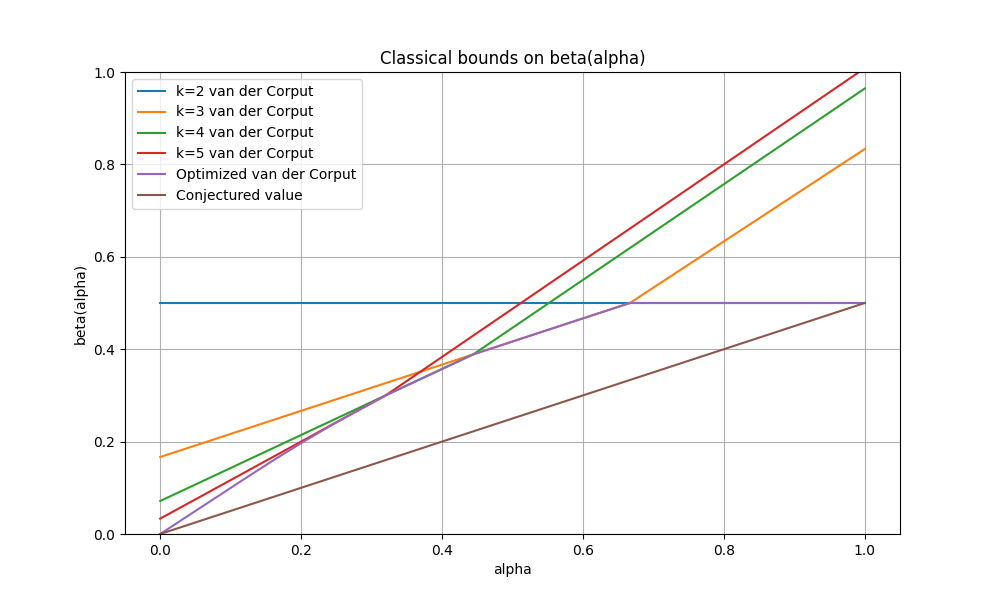
\includegraphics[width=0.5\linewidth]{chapter/van_der_corput_beta.png}
    \caption{The bounds in Proposition \ref{beta-vdc} for $k=2,3,4,5$, compared against the optimized bound in Corollary \ref{vdc-opt}.}
    \label{fig:vdc}
\end{figure}

\begin{figure}
    \centering
    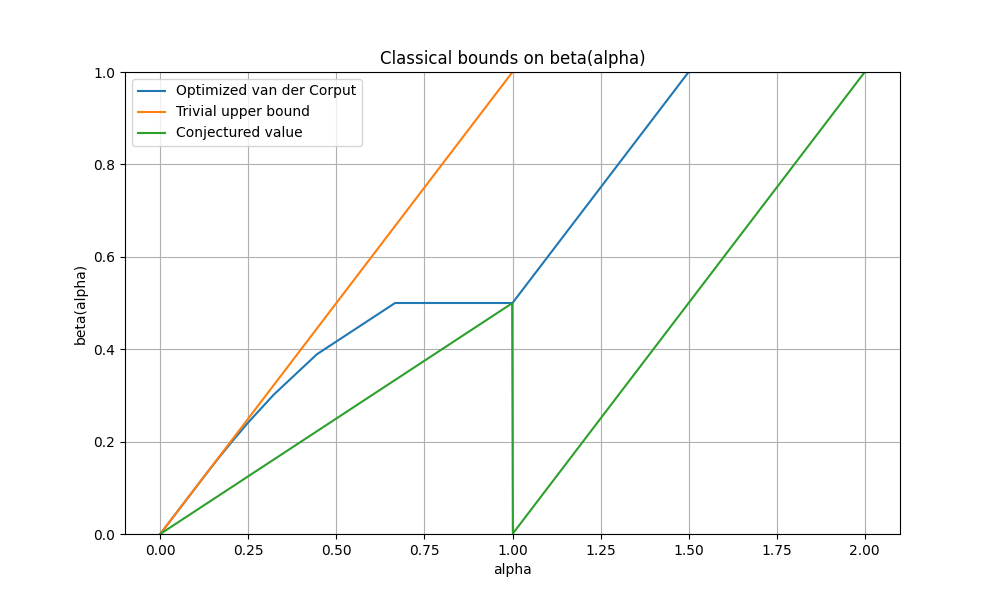
\includegraphics[width=0.5\linewidth]{chapter/van_der_corput_beta_vs_conjectured.png}
    \caption{The bound in Corollary \ref{vdc-opt}, compared against the trivial upper and lower bounds in Lemma \ref{beta-triv}.}
    \label{fig:vdc2}
\end{figure}

We remark that this corollary also follows from Proposition \ref{vdc-class}.



% Exponential sums and the Riemann zeta function II
\begin{theorem}[Watt bound]\label{beta-Watt}\uses{beta-def} For any $3/7 \le \alpha \le 1/2$, one has
    \[
    \beta(\alpha) \le \frac{89}{560} + \frac{1}{2}\alpha.
    \]
    \end{theorem}


\literature
\code{add_beta_bound_watt_1989()}

    \begin{proof}
    See \cite[Theorem~5]{watt_exponential_1989}.
    \end{proof}



% Exponential sums and the Riemann zeta function III
\begin{theorem}[1991 Huxley--Kolesnik bound]\label{beta-HK2}\uses{beta-def}  For any $2/5 \le \alpha \le 1/2$ one has
\[
\beta(\alpha) \le \max\left(\frac{1 + 8\alpha}{22}, \frac{11 + 112\alpha}{158}, \frac{1 + 17\alpha}{22}\right).
\]
\end{theorem}


\literature
\code{add_beta_bound_huxley_kolesnik_1991()}

\begin{proof}
See \cite[Theorem~3]{huxley_exponential_1991}. Note that the paper contains an error, however this result was reinstated with the corrections given in \cite{huxley_exponential_1993_1}.
\end{proof}



% Exponential sums and the Riemann zeta function IV
\begin{theorem}[1993 Huxley bound]\label{beta-Huxley-4}\uses{beta-def} For any $0 \le \alpha \le 49/114$, one has
\[
\beta(\alpha) \le \max\left(\frac{13}{60} + \frac{7}{20}\alpha, \frac{11}{120} + \frac{13}{20}\alpha\right).
\]
Furthermore, for any $49/114 \le \alpha \le 1/2$, one has
\[
\beta(\alpha) \le \frac{89}{570} + \frac{1}{2}\alpha.
\]
\end{theorem}


\literature
\code{add_beta_bound_huxley_1993()}

\begin{proof}
See \cite[Theorem~1]{huxley_exponential_1993}.
\end{proof}


\begin{theorem}[Second 1993 Huxley bound]\label{beta-Huxley-4a}\uses{beta-def} If $0 \leq \alpha \leq 1$, then $\beta(\alpha)$ is bounded by
    \begin{align*}
        \frac{1}{146} (13+94\alpha) & \hbox{ for } \alpha \leq \frac{87}{275} \\
        \frac{1}{244} (11+191\alpha) & \hbox{ for } \frac{87}{275} \leq \alpha \leq \frac{423}{1295} \\
        \frac{1}{1282} (89+908\alpha) & \hbox{ for } \frac{423}{1295} \leq \alpha \leq \frac{227}{601} \\
        \frac{1}{280} (29+173\alpha) & \hbox{ for } \frac{227}{601} \leq \alpha \leq \frac{12}{31} \\
        \frac{1}{128} (4+103\alpha) & \hbox{ for } \frac{12}{31} \leq \alpha \leq 1.
    \end{align*}
\end{theorem}


\literature
\code{add_beta_bound_huxley_1993_3()}

\begin{proof}
See \cite[Theorem~3]{huxley_exponential_1993}.
\end{proof}



\begin{table}[ht]
    \caption{Huxley table 17.1.}
    \centering
    \renewcommand{\arraystretch}{1.2}
    \begin{tabular}{|c|c|c|}
    \hline
    $\beta_0(\alpha)$  & $X$ & $Y$ \\
    \hline
    $\frac{4+39\alpha}{60}$ & $\frac{7}{12}$ & $\frac{517}{873} = 0.5922\dots$ \\
    \hline
    $\frac{29+42\alpha}{120}$ & $\frac{65}{114}$ & $\frac{7}{12} = 0.5833\dots$ \\
    \hline
    $\frac{89+285\alpha}{570}$ & $\frac{49}{114}$ & $\frac{65}{114} = 0.5701\dots$ \\
    \hline
    $\frac{11+78\alpha}{120}$ & $\frac{5}{12}$ & $\frac{49}{114} = 0.4298\dots$ \\
    \hline
    $\frac{13+21\alpha}{60}$ & $\frac{356}{873}$ & $\frac{5}{12} = 0.4166\dots$ \\
    \hline
    $\frac{4+103\alpha}{128}$ & $\frac{12}{31}$ & $\frac{356}{873} = 0.4546\dots$ \\
    \hline
    $\frac{29+173\alpha}{280}$ & $\frac{227}{601}$ & $\frac{12}{31} = 0.3870\dots$ \\
    \hline
    $\frac{89+908\alpha}{1282}$ & $\frac{423}{1295}\dots$ & $\frac{227}{601} = 0.3777\dots$ \\
    \hline
    $\frac{11+191\alpha}{244}$ & $\frac{87}{275}$ & $\frac{423}{1295} = 0.3266\dots$ \\
    \hline
    $\frac{13+94\alpha}{146}$ & $\frac{1424}{4747}$ & $\frac{87}{275} = 0.3163\dots$\\
    \hline
    $\frac{4+235\alpha}{264}$ & $\frac{120}{419}$ & $\frac{1424}{4747}=0.2999\dots$ \\
    \hline
    $\frac{49+1351\alpha}{1614}$ & $\frac{967}{3428}$ & $\frac{120}{419} = 0.2863\dots$ \\
    \hline
    $\frac{29+464\alpha}{600}$ & $\frac{199}{716}$ & $\frac{967}{3428} = 0.2820\dots$ \\
    \hline
    $\frac{89+2243\alpha}{2706}$ & $\frac{19}{74}$ & $\frac{199}{716} = 0.2779\dots$ \\
    \hline
    $\frac{11+428\alpha}{492}$ & $\frac{161}{646}$ & $\frac{19}{74} = 0.2567\dots$ \\
    \hline
    $\frac{13+253\alpha}{318}$ & $\frac{2848}{12173} =0.2339\dots$ & $\frac{161}{646} = 0.2492\dots$ \\
    \hline
    \end{tabular}
    \end{table}\label{huxley-table-1}

    \begin{table}[ht]
        \caption{Huxley table 19.1.}
        \centering
        \renewcommand{\arraystretch}{1.2}
        \begin{tabular}{|c|c|c|}
        \hline
        $\beta_0(\alpha)$  & $X$ & $Y$ \\
        \hline
        $\frac{89+285\alpha}{570}$ & $\frac{106822}{246639}$ & $\frac{139817}{246639}=0.5668\dots$ \\
        \hline
        $\frac{2387+17972\alpha}{27290}$ & $\frac{675}{1574}$ & $\frac{106822}{246639}=0.4331\dots$ \\
        \hline
        $\frac{2819+19177\alpha}{29855}$ & $\frac{699371}{1647930}$ & $\frac{675}{1574}=0.4288\dots$ \\
        \hline
        $\frac{11897+88442\alpha}{134680}$ & $\frac{156527}{370694}$ & $\frac{699371}{1647930}=0.4243\dots$ \\
        \hline
        $\frac{113+897\alpha}{1345}$ & $\frac{263}{638}$ & $\frac{156527}{370694} = 0.4222\dots$ \\
        \hline
        $\frac{491+3624\alpha}{5530}$ & $\frac{143}{349}$ & $\frac{263}{638} = 0.4122\dots$ \\
        \hline
        $\frac{569+1053\alpha}{2800}$ & $\frac{307}{761}$ & $\frac{143}{349} = 0.4097\dots$ \\
        \hline
        $\frac{1273+2484\alpha}{6410}$ & $\frac{68682}{171139}$ & $\frac{307}{761} = 0.4034\dots$ \\
        \hline
        $\frac{4+103\alpha}{128}$ & $\frac{12}{31}$ & $\frac{68682}{171139}=0.4013\dots$ \\
        \hline
        $\frac{29+173\alpha}{280}$ & $\frac{227}{601}=0.3777\dots$ & $\frac{12}{31} = 0.3870\dots$ \\
        \hline
        \end{tabular}
\end{table}\label{huxley-table-2}


% Area, Lattice points and Exponential sums
\begin{theorem}[1996 Huxley table]\label{huxley-table}\uses{beta-def}  One can bound $\beta(\alpha)$ by $\beta_0(\alpha)$ for $X \leq \alpha \leq Y$ for $\beta_0, X, Y$ given by Tables \ref{huxley-table-1}, \ref{huxley-table-2}.
\end{theorem}


\literature
\code{add_beta_bound_huxley_1996()}\\
\code{add_beta_bound_huxley_1996_2()}

\begin{proof} See \cite[Table 17.1, Table 19.2]{huxley_area_1996}.
\end{proof}


    % Exponential sums with a large second derivative
    \begin{theorem}[2001 Huxley--Kolesnik bound]\label{beta-HK}\uses{beta-def}  For any $2/5 \le \alpha \le 1/2$ one has
        $$ \beta(\alpha) \leq \max\left(\frac{7}{80} + \frac{79}{120}\alpha, \frac{3}{32} + \frac{103}{160}\alpha, \frac{9}{40} + \frac{13}{40}\alpha\right).$$
    \end{theorem}

\literature
\code{add_beta_bound_huxley_kolesnik_2001()}

    \begin{proof}
    See \cite[Theorem~1]{huxley_exponential_2001}.
    \end{proof}


%  A Fourth Derivative Test for Exponential Sums
\begin{theorem}[Robert--Sargos bound]\label{beta-RS}\uses{beta-def}  For any $\alpha > 0$ one has
    $$ \beta(\alpha) \leq \max\left( \alpha + \frac{1-4\alpha}{13}, -\frac{7(1-4\alpha)}{13}\right).$$
\end{theorem}

\literature
\code{add_beta_bound_robert_sargos_2002()}

\begin{proof}
See \cite[Theorem~1]{robert_fourth_2002}.
\end{proof}


% An analog of van der Corput’s A4-process for exponential sums
\begin{theorem}[Sargos bound]\label{sargos-bound}\uses{beta-def}  For any $\alpha > 0$ one has
$$ \beta(\alpha) \leq \max\left( \alpha + \frac{1-8\alpha}{204}, -\frac{95(1-8\alpha)}{204}\right)$$
and
$$ \beta(\alpha) \leq \max\left( \alpha + \frac{7(1-9\alpha)}{2640}, -\frac{1001(1-9\alpha)}{2640}\right).$$
\end{theorem}

\literature
\code{add_beta_bound_sargos_2003()}

\begin{proof}
See \cite[Theorems~3, 4]{sargos_analog_2003}.
\end{proof}


% Exponential sums and the Riemann zeta function VI
\begin{theorem}[Huxley bound]\label{beta-Huxley-5}\uses{beta-def} For any $1/3 \le \alpha \le 1/2$, one has
\[
\beta(\alpha) \le \max\left(\frac{37 + 59\alpha}{170}, \frac{63 + 449\alpha}{690}\right).
\]
\end{theorem}

\literature
\code{add_beta_bound_huxley_2005()}

\begin{proof}
See \cite[Proposition~1, Theorem~1]{huxley_exponential_2005}.
\end{proof}


% On the fourth derivative test for exponential sums
\begin{theorem}[Robert bound]\label{beta-R}\uses{beta-def} For any $0 < \alpha \le 3/7$ one has
\[
\beta(\alpha) \le \max\left(\alpha + \frac{1 - 4\alpha}{12}, \frac{11}{12}\alpha\right).
\]
\end{theorem}


\literature
\code{add_beta_bound_robert_2016()}

\begin{proof}
See \cite[Theorem~1]{robert_fourth_2016}.
\end{proof}

\begin{theorem}[Second Robert bound]\label{beta-R2}\uses{beta-def} If $k \geq 4$ and $\alpha \geq -(1-k\alpha) \frac{k-1}{2k-3}$ then
$$ \beta(\alpha) \leq \alpha + \max( \frac{1-k\alpha}{2(k-1)(k-2)}, -\frac{1}{2(k-1)(k-2)}).$$
\end{theorem}

\literature
\code{add_beta_bound_robert_2016_2(Constants.BETA_TRUNCATION)}

\begin{proof} See \cite[Theorem 10]{robert_2016}.
\end{proof}


\begin{theorem}[Heath-Brown bound]\label{beta-HB}\uses{beta-def}  For any $\alpha > 0$ and any natural number $k \geq 3$ one has
$$ \beta(\alpha) \leq \alpha + \max\left( \frac{1-k\alpha}{k(k-1)}, -\frac{\alpha}{k(k-1)}, -\frac{2\alpha}{k(k-1)} - \frac{2(1-k\alpha)}{k^2(k-1)}\right).$$
\end{theorem}

\literature
\code{add_beta_bound_heath_brown_2017(Constants.BETA_TRUNCATION)}

\begin{proof}
See \cite[Theorem~1]{heathbrown_new_2017}.
\end{proof}


\begin{theorem}[Bourgain bound]\label{beta-Bourgain}\uses{beta-def} One has
\[
\beta(\alpha) \le \begin{cases}
\displaystyle\frac{2}{9} + \frac{1}{3}\alpha,&\displaystyle\frac{1}{3} < \alpha \le \frac{5}{12},\\
\\
\displaystyle\frac{1}{12} + \frac{2}{3}\alpha,&\displaystyle\frac{5}{12} < \alpha \le \frac{3}{7},\\
\\
\displaystyle\frac{13}{84} + \frac{1}{2}\alpha,&\displaystyle\frac{3}{7} < \alpha \le \frac{1}{2}.
\end{cases}
\]
\end{theorem}

\literature
\code{add_beta_bound_bourgain_2017()}

\begin{proof}
See \cite[Equation~(3.18)]{bourgain_decoupling_2017}.
\end{proof}

\begin{theorem}[Heath-Brown 2020 bound]\label{beta-hb-2020}\uses{beta-def}\cite[Theorem 11.2]{demeter_small_2020}  If $\alpha$ is fixed with $1 \leq 4\alpha-1 \leq 2$ (i.e., $1/2 \leq \alpha \leq 3/4$), then
$$ \beta(\alpha) \leq \max( \alpha(1 - \frac{4\alpha-1}{4(4\alpha-1)+8}), \frac{8}{9} \alpha).$$
\end{theorem}

{\bf TODO: implement this in python}

\begin{theorem}[Combined bound]  For $X \leq \alpha \leq Y$, one has $\beta(\alpha) \leq \beta_0(\alpha)$, where $\beta_0, X, Y$ are given by Table \ref{huxley_table_ranges}.
\end{theorem}

\begin{proof} See \cite[Table 3]{trudgian-yang}.
\end{proof}

\begin{table}[ht]
    \def\arraystretch{1.3}
    \centering
    \caption{Bounds on $\beta(\alpha)$ of the form $\beta(\alpha) \le \beta_0(\alpha), \;(X \le \alpha \le Y)$}
    \begin{tabular}{|c|c|c|c|}
    \hline
    $\beta_0(\alpha)$ & $X$ & $Y$ & Reference\\
    \hline
    $ \frac{13}{414} + \frac{359}{414} \alpha $ & $ 0 $ & $ \frac{2848}{12173} = 0.2339\ldots $ & Exponent pair $A^2(\frac{13}{84}, \frac{55}{84})$\\
    \hline
    $\frac{13}{318} + \frac{253}{318} \alpha$ & $\frac{2848}{12173}$ & $\frac{161}{646} = 0.2492\ldots$ & Table \ref{huxley-table-1}\\
    \hline
    $\frac{11}{492} + \frac{107}{123} \alpha$ & $\frac{161}{646}$ & $\frac{19}{74} = 0.2567\ldots$ & Table \ref{huxley-table-1}\\
    \hline
    $ \frac{89}{2706} + \frac{2243}{2706} \alpha $ & $ \frac{19}{74} $ & $ \frac{199}{716} = 0.2779\ldots $ & Table \ref{huxley-table-1}\\
    \hline
    $ \frac{29}{600} + \frac{58}{75} \alpha $ & $ \frac{199}{716} $ & $ \frac{967}{3428} = 0.2820\ldots $ & Table \ref{huxley-table-1}\\
    \hline
    $ \frac{49}{1614} + \frac{1351}{1614} \alpha $ & $ \frac{967}{3428} $ & $ \frac{120}{419} = 0.2863\ldots $ & Table \ref{huxley-table-1}\\
    \hline
    $ \frac{1}{66} + \frac{235}{264} \alpha $ & $ \frac{120}{419} $ & $ \frac{1328}{4447} = 0.2986\ldots $ & Table \ref{huxley-table-1}\\
    \hline
    $ \frac{13}{194} + \frac{139}{194} \alpha $ & $ \frac{1328}{4447} $ & $ \frac{104}{343} = 0.3032\ldots $ & Exponent pair $A(\frac{13}{84}, \frac{55}{84})$\\
    \hline
    $ \frac{13}{146} + \frac{47}{73} \alpha $ & $ \frac{104}{343} $ & $ \frac{87}{275} = 0.3163\ldots $ & Table \ref{huxley-table-1}\\
    \hline
    $ \frac{11}{244} + \frac{191}{244} \alpha $ & $ \frac{87}{275} $ & $ \frac{423}{1295} = 0.3266\ldots $ & Table \ref{huxley-table-1}\\
    \hline
    $ \frac{89}{1282} + \frac{454}{641} \alpha $ & $ \frac{423}{1295} $ & $ \frac{227}{601} = 0.3777\ldots $ & Table \ref{huxley-table-1}\\
    \hline
    $ \frac{29}{280} + \frac{173}{280} \alpha $ & $ \frac{227}{601} $ & $ \frac{12}{31} = 0.3870\ldots $ & Table \ref{huxley-table-1}\\
    \hline
    $ \frac{1}{32} + \frac{103}{128} \alpha $ & $ \frac{12}{31} $ & $ \frac{1508}{3825} = 0.3942\ldots $ & Table \ref{huxley-table-1}\\
    \hline
    $ \frac{18}{199} + \frac{521}{796} \alpha $ & $ \frac{1508}{3825} $ & $ \frac{62831}{155153} = 0.4049\ldots $ & Sargos \cite{sargos_points_1995}\\
    \hline
    $ \frac{569}{2800} + \frac{1053}{2800} \alpha $ & $ \frac{62831}{155153} $ & $ \frac{143}{349} = 0.4097\ldots $ & Table \ref{huxley-table-2}\\
    \hline
    $ \frac{491}{5530} + \frac{1812}{2765} \alpha $ & $ \frac{143}{349} $ & $ \frac{263}{638} = 0.4122\ldots $ & Table \ref{huxley-table-2}\\
    \hline
    $ \frac{113}{1345} + \frac{897}{1345} \alpha $ & $ \frac{263}{638} $ & $ \frac{1673}{4038} = 0.4143\ldots $ & Table \ref{huxley-table-2}\\
    \hline
    $ \frac{2}{9} + \frac{1}{3} \alpha $ & $ \frac{1673}{4038} $ & $ \frac{5}{12} = 0.4166\ldots $ & Theorem \ref{beta-Bourgain}\\
    \cline{1-3}
    $ \frac{1}{12} + \frac{2}{3} \alpha $ & $ \frac{5}{12} $ & $ \frac{3}{7} = 0.4285\ldots $ & Theorem \ref{beta-Bourgain}\\
    \cline{1-3}
    $ \frac{13}{84} + \frac{1}{2} \alpha $ & $ \frac{3}{7} $ & $ \frac{1}{2}$ & Theorem \ref{beta-Bourgain}\\
    \hline
    \end{tabular}
    \label{huxley_table_ranges}
    \end{table}

{\bf TODO: implement this in Python}

{\bf TODO: state the Sargos result above as a lemma and a line of python code}

{\bf TODO: provide a graphic of the best bounds available of beta, compared against the classical van der Corput bounds}
